\documentclass[thesis=M,english,hidelinks]{FITthesis}[2012/10/20]

\usepackage[utf8]{inputenc} % LaTeX source encoded as UTF-8
\usepackage{dirtree} %directory tree visualisation
\usepackage{graphicx} %graphics files inclusion
\usepackage{todonotes}
\usepackage{multicol}
\usepackage[acronym,nonumberlist,toc,numberedsection=autolabel,nopostdot]{glossaries}

\newcommand*{\fullref}[1]{\hyperref[{#1}]{\autoref*{#1}: \textit{\nameref*{#1}}}}

% % % % % % % % % % % % % % % % % % % % % % % % % % % % % % 
% FORMAL STUFF
% % % % % % % % % % % % % % % % % % % % % % % % % % % % % % 

\department{Department of Software Engineering}
\title{Applying the Normalized Systems Theory on Microservice Architecture}
\authorGN{Vincenc} %author's given name/names
\authorFN{Kolařík} %author's surname
\author{Vincenc Kolařík} %author's name without academic degrees
\authorWithDegrees{Bc. Vincenc Kolařík} %author's name with academic degrees
\supervisor{Ing. Robert Pergl, Ph.D.}
\placeForDeclarationOfAuthenticity{Prague}
\declarationOfAuthenticityOption{1} %select as appropriate, according to the desired license (integer 1-6)

% % % % % % % % % % % % % % % % % % % % % % % % % % % % % % 
% ABSTRACT & KEYWORDS
% % % % % % % % % % % % % % % % % % % % % % % % % % % % % % 

\acknowledgements{Thanks to my family and girlfriend, Tamara, for all the patience and care. Thanks to my thesis supervisor, Robert, for everything he taught me.}

\abstractEN{Summarize the contents and contribution of your work in a few sentences in English language.Summarize the contents and contribution of your work in a few sentences in English language.Summarize the contents and contribution of your work in a few sentences in English language.Summarize the contents and contribution of your work in a few sentences in English language.Summarize the contents and contribution of your work in a few sentences in English language.Summarize the contents and contribution of your work in a few sentences in English language.Summarize the contents and contribution of your work in a few sentences in English language.Summarize the contents and contribution of your work in a few sentences in English language.Summarize the contents and contribution of your work in a few sentences in English language.}

\abstractCS{V n{\v e}kolika v{\v e}t{\' a}ch shr{\v n}te obsah a p{\v r}{\' i}nos t{\' e}to pr{\' a}ce v {\v c}esk{\' e}m jazyce.V n{\v e}kolika v{\v e}t{\' a}ch shr{\v n}te obsah a p{\v r}{\' i}nos t{\' e}to pr{\' a}ce v {\v c}esk{\' e}m jazyce.V n{\v e}kolika v{\v e}t{\' a}ch shr{\v n}te obsah a p{\v r}{\' i}nos t{\' e}to pr{\' a}ce v {\v c}esk{\' e}m jazyce.V n{\v e}kolika v{\v e}t{\' a}ch shr{\v n}te obsah a p{\v r}{\' i}nos t{\' e}to pr{\' a}ce v {\v c}esk{\' e}m jazyce.V n{\v e}kolika v{\v e}t{\' a}ch shr{\v n}te obsah a p{\v r}{\' i}nos t{\' e}to pr{\' a}ce v {\v c}esk{\' e}m jazyce.V n{\v e}kolika v{\v e}t{\' a}ch shr{\v n}te obsah a p{\v r}{\' i}nos t{\' e}to pr{\' a}ce v {\v c}esk{\' e}m jazyce.V n{\v e}kolika v{\v e}t{\' a}ch shr{\v n}te obsah a p{\v r}{\' i}nos t{\' e}to pr{\' a}ce v {\v c}esk{\' e}m jazyce.V n{\v e}kolika v{\v e}t{\' a}ch shr{\v n}te obsah a p{\v r}{\' i}nos t{\' e}to pr{\' a}ce v {\v c}esk{\' e}m jazyce.V n{\v e}kolika v{\v e}t{\' a}ch shr{\v n}te obsah a p{\v r}{\' i}nos t{\' e}to pr{\' a}ce v {\v c}esk{\' e}m jazyce.V n{\v e}kolika v{\v e}t{\' a}ch shr{\v n}te obsah a p{\v r}{\' i}nos t{\' e}to pr{\' a}ce v {\v c}esk{\' e}m jazyce.V n{\v e}kolika v{\v e}t{\' a}ch shr{\v n}te obsah a p{\v r}{\' i}nos t{\' e}to pr{\' a}ce v {\v c}esk{\' e}m jazyce.V n{\v e}kolika v{\v e}t{\' a}ch shr{\v n}te obsah a p{\v r}{\' i}nos t{\' e}to pr{\' a}ce v {\v c}esk{\' e}m jazyce.V n{\v e}kolika v{\v e}t{\' a}ch shr{\v n}te obsah a p{\v r}{\' i}nos t{\' e}to pr{\' a}ce v {\v c}esk{\' e}m jazyce.}

\keywordsCS{Replace with comma-separated list of keywords in Czech.}
\keywordsEN{Replace with comma-separated list of keywords in English.}

% % % % % % % % % % % % % % % % % % % % % % % % % % % % % % 
% ACRONYMS
% % % % % % % % % % % % % % % % % % % % % % % % % % % % % % 
\makeglossaries
\newacronym{CVUT}{{\v C}VUT}{{\v C}esk{\' e} vysok{\' e} u{\v c}en{\' i} technick{\' e} v Praze}
\newacronym{FIT}{FIT}{Fakulta informa{\v c}n{\' i}ch technologi{\' i}}

\newacronym{API}{API}{application programming interface}
\newacronym{AWS}{AWS}{Amazon Web Services}
\newacronym{BE}{BE}{back-end}
\newacronym{CAP}{CAP}{consistency, availability, partition tolerance (theorem)}
\newacronym{CI}{CI}{continuous integration}
\newacronym{CD}{CD}{continuous delivery}
\newacronym{DAO}{DAO}{data access object}
\newacronym{DB}{DB}{database}
\newacronym{DBMS}{DBMS}{database management system}
\newacronym{DDD}{DDD}{domain driven design}
\newacronym{DRY}{DRY}{don't repeat yourself}
\newacronym{DTO}{DTO}{data transfer object}
\newacronym{EA}{EA}{enterprise architecture}
\newacronym{ESB}{ESB}{enterprise service bus}
\newacronym{FE}{FE}{front-end}
\newacronym{FP}{FP}{functional programming}
\newacronym{IOT}{IoT}{internet of things}
\newacronym{IPC}{IPC}{inter-process communication}
\newacronym{IT}{IT}{information technology}
\newacronym{JSON}{JSON}{JavaScript object notation}
\newacronym{MAPE}{MAPE}{monitoring, analysis, planning, execution}
\newacronym{MSA}{MSA}{microservice architecture}
\newacronym{MS}{MS}{microservice}
\newacronym{MVC}{MVC}{Model-View-Controller architecture}
\newacronym{MVVM}{MVVM}{Model-View-ViewModel architecture}
\newacronym{NS}{NS}{Normalized Systems theory}
\newacronym{OOP}{OOP}{object oriented programming}
\newacronym{ORM}{ORM}{object-relational mapping}
\newacronym{POJO}{POJO}{plain old Java object}
\newacronym{RD}{R\&D}{research and development}
\newacronym{REST}{REST}{representational state transfer}
\newacronym{RPC}{RPC}{remote procedure call}
\newacronym{SA}{SA}{software architecture}
\newacronym{SOA}{SOA}{service-oriented architecture}
\newacronym{SOAP}{SOAP}{simple object access protocol}
\newacronym{SW}{SW}{software}
\newacronym{VM}{VM}{virtual machine}
\newacronym{XML}{XML}{extensible markup language}

%%%%%%%%%%%%%%%%%%%%%%%%%%%%%%%%%%%%%%%%%%%%%%%%%%%%%%%%%%%%
%%%%%%%%%%%%%%%%%%%%%%%%%%%%%%%%%%%%%%%%%%%%%%%%%%%%%%%%%%%%
%%                                                        %%
%%                      THE DOCUMENT                      %%
%%                                                        %%
%%%%%%%%%%%%%%%%%%%%%%%%%%%%%%%%%%%%%%%%%%%%%%%%%%%%%%%%%%%%
%%%%%%%%%%%%%%%%%%%%%%%%%%%%%%%%%%%%%%%%%%%%%%%%%%%%%%%%%%%%
\begin{document}

% % % % % % % % % % % % % % % % % % % % % % % % % % % % % % 
% 
% INTRODUCTION
% 
% % % % % % % % % % % % % % % % % % % % % % % % % % % % % % 
\setsecnumdepth{part}
\chapter{Introduction}
\todo[inline,size=\Large]{Missing whole chapter}
\begin{verbatim}
motivace

- same goals, different approach
- microservices = craftmanship
- NS theory of systems
- distributed 
    
- loose coupling high cohesion

- modularity, granularity, evolvability
- evolvability, adaptation to change

    
\end{verbatim}

Widely used throughout the industry by leading companies \cite{ms-who-is-using}.

\setsecnumdepth{all}

% % % % % % % % % % % % % % % % % % % % % % % % % % % % % % 
% 
% GOALS AND APPROACH
% 
% % % % % % % % % % % % % % % % % % % % % % % % % % % % % % 
\chapter{Goals and Approach}
\section{Goals}
According to~a~thesis assignment the~following goals were set:
\begin{itemize}
	\item Analyze the current state-of-the-art design methods and industrial applications of microservice architecture.
	\item Identify key features and the most significant challenges encountered in~the~industry.
	\item Discuss compliance of the currently used methods with \acrlong{NS} and explore possibilities for improvements using \acrshort{NS}. 
	\item Formulate guidelines for designing microservices based on the results from the previous chapter, discuss them and demonstrate them on~a~case study if reasonable.
\end{itemize}

\section{Approach}
Microservices architecture is an \acrfull{EA} pattern. \acrshort{EA} could be analyzed in enormously broad context, spanning from business-IT alignment, through \acrshort{SW} development methodologies to a choice of programming languages. This section discusses boundaries for this thesis to make the topic reasonably narrow without overlooking the quintessence of \acrlong{MSA}.

\subsection{Organizational Aspects}
Microservices are often valued for their positive effects on organizations and teams of engineers creating them. Development of end-to-end features and operational responsibility fosters DevOps culture \cite{devops-what-is}. Code ownership and cross-functional teams cultivate team spirit and nurture motivation of developers \cite{ms-fow-new-term-def, ms-modelling-with-petter, ms-building-ms}.

There's also a sociological observation called \textit{Conway's law} that states:
\begin{quote}
    Any organization that designs a system (defined broadly) will produce a design whose structure is a copy of the organization's communication structure.~\cite{conways-law}
\end{quote}

The bi-directional influence between software architecture and the organization that creates it is a remarkable topic, and it would be unwise to ignore it while running a business. Despite that, it will be ignored in this thesis, as it would broaden its scope excessively. The \acrshort{NS} literature \cite{ns-recreating, ns-toward-general-theory} has the same attitude and avoids discussion how the organization influences the \acrshort{SW} and vice versa.

\subsection{Performance aspects}
The \acrlong{NS} describes a set of laws which, if applied strictly, guarantee a system to be free from combinatorial effects, i.e., to be indefinitely evolvable. Until now, the industrial \acrlong{SW} projects \cite{ns-it-isnt-different, ns-exploring-defence} are focused on the evolvability of the \acrshort{SW} artifact and doesn't value any other non-functional requirement as much as evolvability.

On the other hand, \acrlong{MS} came into being due to the need for performance and scalability \cite{ms-building-ms, ms-evolutionary-arch}. The evolvability aspect is never more important that those two mentioned. Therefore this thesis will respect this order and will not sacrifice performance and scalability for the sake of evolvability.

\subsection{Libraries, frameworks and other 3rd party technologies}
Microservices are the present-day buzzword
    - turbulent times, new frameworks emerging and be abandoned every day
    - https://github.com/mfornos/awesome-microservices not an extensive list of tech, but will suffice
    - don't bother with choosing and comparing particular 3rd party tech, too small detail
    - exctract the principcle and compare that

\subsection{User Interface and }
\begin{verbatim}
    - tons of presentations layers, frontends, desktop apps, mobile apps, watch apps and gadgets 
    - end with external API \ref{sec:ext_api}
\end{verbatim}

\subsection{General Rules}
In an~effort to~make this work conceptually coherent, there were defined essential principles with which this thesis is created:
\begin{enumerate}
    \item Avoid discussion how organization influences the \acrshort{SW} and vice versa.
    \item Do not sacrifice performance and scalability for the sake of evolvability.
    \item When recommending to use an existing technology, extract the principle and recommend that 
\end{enumerate}

\section{Thesis Structure and Tasks}
To fulfill the goals of this thesis the following finer-grain task was defined. The~final structure of~this work is derived from this task list.
\begin{enumerate}
% 	\item Provide an~overview of~utilized theories and concepts (Chapter~\textit{\nameref{sec:theoretical_background}})
% 	\begin{itemize}
% 		\item Introduce key concepts of~\acrlong{NS}
% 		\item Describe the key principles and motivation for \acrlong{MSA}
% 	\end{itemize}

	\item Perform a literature review on \acrshort{MS} and on application of \acrshort{NS} to \acrshort{MS} and/or related architecture styles and patterns
	\begin{itemize}
		\item[$\Rightarrow$] \fullref{sec:literature_review}
	\end{itemize}
	
	\item Analyze the \acrlong{MSA}
	\begin{itemize}
        \item Extract the essential concepts of state-of-the-art design of \acrshort{MS}
		\item Identify key concerns in \acrshort{MS} design and implementation
		\item[$\Rightarrow$] \fullref{sec:msa_analysis}
	\end{itemize}

	\item Examine compliance of \acrlong{MSA} to \acrlong{NS}
	\begin{itemize}
		\item Discuss the architectural patterns and principles using \acrlong{NS}
		\item Apply the \textit{Design Theorems for Stable Software} \cite{ns-towards-evolvable} to the essential concepts from previous chapter
		\item[$\Rightarrow$] \fullref{sec:msa_compliance}
	\end{itemize}	

	\item Summarize design guidelines for \acrshort{MSA}
	\begin{itemize}
		\item Provide concise and comprehensive overview of formulated guidelines
		\item Demonstrate guidelines on suitable case study
		\item[$\Rightarrow$] \fullref{sec:guidelines}
	\end{itemize}
	
	\item Summarize successes and failures
	\begin{itemize}
		\item[$\Rightarrow$] chapter: \textit{\nameref{sec:conclusion}}
	\end{itemize}
\end{enumerate}

% % % % % % % % % % % % % % % % % % % % % % % % % % % % % % 
% 
% Theoretical Background
% 
% % % % % % % % % % % % % % % % % % % % % % % % % % % % % % 
\chapter{Theoretical Background}
\label{sec:theoretical_background}

% 
% Introduction to Normalized Systems
% 
\section{Introduction to Normalized Systems}
\acrfull{NS} is a theoretical framework designed to engineer systems (in its broad meaning) to be able to absorb a set of anticipated changes in an infinite period. The ability to absorb changes ---~\textit{evolvability}~--- is the essential property of studied systems. The theory formulates a set of~\textit{rules of evolvability} backed by formal proofs (more in section \ref{sec:evolvability_rules}).

\subsection{Ongoing Research}
The~theory is being developed at the University of~Antwerp, the~department Management Information Systems of~the~faculty Applied Economics. Due to its success, the~authors, Jan Verelst and Herwig Mannaert, have established the~Normalized Systems Institute for further applied research in the \acrshort{SW} industry.

Although the theory originated in a narrow field --- \acrlong{SW} development, it has been generalized and now is being applied to wide range of various disciplines: from business process modeling through legal documents to first thoughts on civil engineering.~\cite{ns-towards-evolvable}

Due to the focus of this thesis, \acrlong{NS} will be explained on the domain of \acrlong{SW} development.

\subsection{Essential Principles}
\label{sec:evolvability_rules}

\begin{figure}[t]
  \centering
    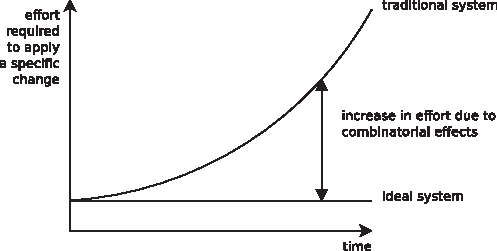
\includegraphics{images/Combinatorial_effects_explained.pdf}
   	\caption{Combinatorial effects explained}
    \label{fig:combinatorial_effects}
\end{figure}

The authors of \acrlong{NS} state the contemporary \acrshort{IT} problems are manifestations of~fundamental flaws in~currently used \acrshort{SW} development methodologies. The Achilles' heel is the evolvability --- adding new features to~existing code base generates \emph{combinatorial effects} (or \textit{instabilities} in newer literature, e.g. \cite{ns-toward-general-theory}), that lead to a~growth of~overall system complexity (see fig. \ref{fig:combinatorial_effects}~\cite{ns-recreating}). Such effects cause to increase the cost of future changes and decrease overall software quality.\cite{ns-recreating}

Initial idea was first uttered by Manny Lehman in~1980:
\begin{quote}
    As an~evolving program is continually changed, its complexity, reflecting deteriorating structure, increases unless work is done to~maintain or reduce it.~\cite{lehman-1980-programs}
\end{quote}

In spite of~that, \acrlong{NS} strive to fulfill the dream articulated by Douglas McIlroy in~1968:
\begin{quote}
    Expect families of~routines to~be constructed on rational principles so that families fit together as building blocks. In short, [the user] should be able safely to~regard components as black boxes.~\cite{mcilroy-1968-mass-software}
\end{quote}

\acrshort{NS} assume that a~change introduced to~a~system is a natural and unavoidable phenomenon. Therefore all rules and principles are designed to~accommodate that fact. The~theory defines a set of~guidelines on how to~engineer the~\acrlong{SW} architecture as a structure of~highly independent modules, which can be added, removed or changed separately. Sufficiently granular architecture will suppress all combinatorial effects during evolution of~the~system.

The~normalized design theorems require a strict separation of~data and actions manipulating that data. Such segregation might be controversial as it contradicts the~essence of~\acrfull{OOP}, which postulates that data and related actions belong into one entity --- a \textit{class}.

% 
% Design Theorems of Stable Software
% 
\section{Design Theorems of Stable Software}
\label{sec:theorems}
This section introduces the four rules of~software evolvability --- \textit{the design theorems of stable software}, which are the building blocks of~\acrshort{NS} theory. An experienced software developer will recognize these rules as they originate from a heuristic design knowledge. The value added by \acrshort{NS} is the theoretical proofs which promote these practical experiences to~defensible theorems. (The proofs are omitted for brevity, but can be found in \cite{ns-recreating, ns-toward-general-theory}.)

\subsection{The Four Theorems}
The \acrshort{NS} theory can prove the system is free from instabilities if and only if the system complies to all the design theorems. Therefore the following postulate is set as an ultimate goal:
\begin{quote}
    An evolving information system should not have \textit{instabilities} (\textit{combinatorial effects}): a bounded amount of additional functional requirements cannot lead to an unbounded amount of additional (versions of) software primitives.~\cite{ns-toward-general-theory}
\end{quote}

\subsubsection{Separation of~Concerns}
\begin{quote}
A processing function can only contain a single task in order to achieve stability.~\cite{ns-toward-general-theory}
\end{quote}

This theorem implies the identification and separation of~every single \textit{task}. Correct separation of~tasks will induce \emph{separation of~concerns} in~the~big picture.

Separation of concerns is a~widely used \emph{best practice} among software architects. However, it is very vaguely formulated. Current manifestations in~software development include for example \emph{multi-tier architectures} (e.g., \acrshort{MVC}, \acrshort{MVVM}) or use of~an~\emph{integration bus} for inter-process communication.

\subsubsection{Data Version Transparency}
\begin{quote}
A structure that is passed through the interface of a processing function needs to exhibit version transparency in order to achieve stability.~\cite{ns-toward-general-theory}
\end{quote}

Data version transparency is an instrument to~cope with an addition or removal a~\emph{data field} in~entity. It implies encapsulation of~the~data fields. Wrapping the~data entity allows co-existence of~various versions of~such entity.

An example from \acrshort{OOP}: data version transparency can be easily achieved by using exclusively the \textit{0-parameter constructor} for instantiation and \emph{accessor methods} for the attribute access (e.g., a \acrshort{POJO}). In that case, all internal data fields are hidden and addition of a new one does not cause processing method to fail.

\subsubsection{Action Version Transparency}
\begin{quote}
A processing function that is called by another processing function, needs to exhibit version transparency in order to achieve stability.~\cite{ns-toward-general-theory}
\end{quote}

Analogously to~previous theorem, various versions of~data entities need to~co-exist in~single system.

This can be achieved by using wrapper functions in procedural programming or by using polymorphism in \acrshort{OOP}.

\subsubsection{Separation of~States}
\begin{quote}
Calling a processing function within another processing function, needs to exhibit state keeping in order to achieve stability.~\cite{ns-toward-general-theory}
\end{quote}

It is a~formalization of~instinctive \emph{avoiding the~transition to an undefined state}. When a~state is kept for every call of a processing function, the~whole system behaves as a~deterministic state machine. This eliminates the~need for complicated recovery from undefined error states.

An example of a~manifestation of~this design theorem is a~database transaction mechanism. The~commit (rollback) action guarantees atomic transition from one defined state to~another.

\subsection{Impacts on Software Development}
The postulate in section \ref{sec:theorems} implies all the \textit{design theorems for stable software} must be consistently followed. The~\acrshort{SW} artifact must be free of~instabilities at compile time, deployment time and run time. It requires the~code base to~be entirely error free, which is not an~easy task to~achieve.

Other inconveniences are inevitably encountered during the development of \acrshort{SW} according to \acrshort{NS}. For example the~\emph{data} and \emph{action version transparency} rules also imply a~lot of~\textit{boilerplate} (non-logic) code (e.g., wrapper classes, accessor methods). For a~human programmer writing code complying with \acrshort{NS} is annoying and frustrating.

On the~other hand, \acrshort{NS} presents a~set of~\emph{software design patterns} (described in \cite{ns-recreating}) which could be easily produced via code generation. The generated boilerplate code skeleton is then enriched with custom code containing business logic and algorithms. In case the skeleton itself is introduced to a change, the custom code is \textit{harvested} and then \textit{re-injected} back to the fully re-generated skeleton.~\cite{vk-bp}

The code generation approach remedies the developers' disgruntlement for sure. However, it requires the development of sophisticated tooling to get the fully \acrshort{NS}-compliant \acrlong{SW} working. The only known implementation --- the \textit{NSX Expanders}\footnote{https://normalizedsystems.org/tools/} --- is capable of production of remarkably granular, yet still \textit{monolithic} applications.

This thesis is an attempt to broaden the application of \acrlong{NS} to a domain of distributed software architectures.

% 
% Software Architecture
% 
\section{Introduction to Software Architecture}
As time goes by, the size and complexity of a software system grow, the design questions soon grow beyond algorithms and data structures. The new problem of the overall system design emerges.

When the problem is untreated, applications soon become tightly coupled, brittle and increasingly difficult to change. Even experienced team of developers without a vision resort to the prosaic layered architecture pattern also known as the \textit{n-tier architecture}, creating implicit layers by separating source-code modules into packages. A result of this practice often is a collection of poorly organized source code, modules and components lack clear borders, responsibilities, and relationships with each other. This primeval architecture style is mockingly called a \textit{the big ball of mud}~\cite{big-ball-mud}.

\subsection{Formal Definition}
Obviously, the topic of \acrfull{SA} is frequently discussed. There are many conferences organized by respected organizations (e.g., IEEE International Conference on Software Architecture\footnote{http://icsa-conferences.org/}, O'Reilly Software Architecture Conference\footnote{https://conferences.oreilly.com/software-architecture/}), many people bear a job title \textit{Software Architect} or \textit{Solutions Architect}\footnote{https://www.glassdoor.com/}. Despite all that, there are many definitions of \textit{software architecture}, and none of them is considered universal.

For example, the IEEE Computer Society defines software architecture as:
\begin{quote}
    [Software] Architecture is the fundamental organization of a system embodied in its components, their relationships to each other, and to the environment, and the principles guiding its design and evolution.~\cite{std-ieee-arch}
\end{quote}

One of the pioneers of \acrlong{SA}, Len Bass, defines this complex discipline as:
\begin{quote}
    The software architecture of a computing system is the set of structures needed to reason about the system, which comprise software elements, relations among them, and properties of both.~\cite{documenting-sw-arch}
\end{quote}

After introducing these two definitions, the problem of \acrshort{SA} seem to be highly abstract and difficult. It is clear there's a need of an instrument, that will help break down this complex domain. Such an instrument is featured in the next chapter.

% 
% 4+1 View Model of Architecture
% 
\section{4+1 View Model of Architecture}
The \textit{4+1 View Model} was designed by Philippe Kruchten as a tool \textit{describing the architecture of software-intensive systems, based on the use of multiple, concurrent views}.~\cite{arch-41-views}

Architects may use the four views to systematically depict the miscellaneous \acrshort{SW} elements and the fifth view --- scenarios (or \textit{use cases} in contemporary terminology) which \textit{illustrate} or \textit{animate} the static system.

The view model is \textit{generic}. It doesn't prescribe any particular notation for the different perspectives, or any set of available \textit{architectural patterns} or \textit{styles}, hence allowing the multiple styles coexist in one system.

\begin{figure}
  \centering
    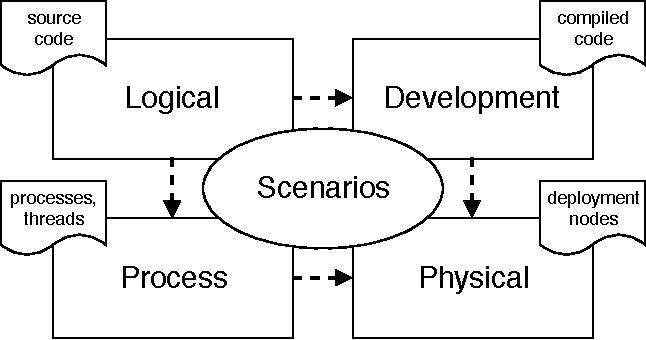
\includegraphics{images/4+1_view.pdf}
    \caption{4+1 View Model of Architecture}
    \label{fig:arch-41-view}
\end{figure}

\subsection{Views Description}
\label{sec:41-views-description}

\begin{itemize}
    \item \textbf{Logical view} describes the elementary code fragments produced by developers --- classes, funtions, configuration files, etc.
    \begin{itemize}
        \item \textbf{Components:} class (\acrshort{OOP}), function (\acrshort{FP})
        \item \textbf{Connectors:} association, inheritance, composition
        \item \textbf{Stakeholders:} end-user
        \item \textbf{Concerns:} functionality
    \end{itemize}
    
    \item \textbf{Development view} depics the artefacts of a packaged runnable code. It describes modules (e.g., a JAR file) and components (e.g., a WAR archive or executable JAR) components and dependencies among them.
    \begin{itemize}
        \item \textbf{Components:} compiled \acrshort{SW} artefacts
        \item \textbf{Connectors:} compile-time dependencies
        \item \textbf{Stakeholders:} developer, operations engineer
        \item \textbf{Concerns:} modularity, code reuse, portability, deployable artefact boundaries
    \end{itemize}
    
    \item \textbf{Process view} represents components at runtime.
    \begin{itemize}
        \item \textbf{Components:} processes
        \item \textbf{Connectors:} inter-process communication (e.g., \acrshort{REST}/\acrshort{SOAP}/\acrshort{RPC} call) 
        \item \textbf{Stakeholders:} developer, operations engineer
        \item \textbf{Concerns:} performance, availability, fault-tolerance, data integrity
    \end{itemize}
    
    \item \textbf{Physical view} describes how the running deployed artifacts are mapped to \textit{deployment nodes}.
    \begin{itemize}
        \item \textbf{Components:} nodes (i.e. containers, \acrshort{VM}s, physical machines)
        \item \textbf{Connectors:} network interfaces
        \item \textbf{Stakeholders:} operations engineer
        \item \textbf{Concerns:} scalability, performance, availability
    \end{itemize}
    
    \item \textbf{Scenarios} are detailed recipes describing actions across the whole application. This view is redundant to the previous four --- therefore marked as \textit{+1} --- but serves as a validation mechanism for the whole architectural vision.
    \begin{itemize}
        \item \textbf{Components:} step-by-step scenarios
        \item \textbf{Connectors:} use-case dependencies
        \item \textbf{Stakeholders:} end-user, developer, QA engineers
        \item \textbf{Concerns:} understandability
    \end{itemize}
\end{itemize}

\subsection{Relations between views}
The four views are not fully independent or orthogonal. Elements of one view must relate to elements in other views, otherwise, the model has some inconsistencies (e.g., non deployed code artifacts, not utilized or inaccessible \acrshort{VM}s). Directions of those relations --- \textit{mappings} --- are shown in \ref{fig:arch-41-view} using the black arrows.

Although every \acrlong{SA} could be viewed from all of those four viewpoints, it is not always necessary to draw all of them to describe the architecture sufficiently. For example, a simple web application running on a single machine with an embedded database does not need a physical view, as it would depict just one machine hosting one process. On the opposite side, systems with millions of lines of code may require logical view diagrams containing thousands of classes and packages. This view would require a high level of abstraction to be understandable. The abstractions could become almost identical to the development view, and therefore render the logical view redundant.

The scenarios are always useful since they contain information about the purpose of the application --- the business value.

\section{Architectural Styles}
The term \textit{architectural style} is in similar manner used in civil engineering. Building were designed in \textit{renaissance}, \textit{functionalism} or \textit{brutalism} styles. All buildings of the particular style were different, yet they shared the same materials, had similar properties (e.g., aesthetics, hygiene), and they were build to fulfill the same ideals.

That is surprisingly close to how it applies to software --- the applications of particular style are built using the same set of elements and relations between them (e.g., classes and their composition), they exhibit the same properties (e.g., layering, modularity) and are build to fulfill the same non-functional requirements (e.g., high availability, rapid evolvability).

There is a often-cited definition of architectural style by David Garlanand and Mary Shaw published in 1994:
\begin{quote}
An architectural style, then, defines a family of such systems in terms of a pattern of structural organization. More specifically, an architectural style determines the vocabulary of components and connectors that can be used in instances of that style, together with a set of constraints on how they can be combined.~\cite{sa-intro-garlan-shaw}
\end{quote}

Architectural styles are usually characterized only from a single view. For example, a \acrfull{MVC} application is defined in logical view as a trio of interacting components, each with its defined responsibility and function. \acrshort{MVC} doesn't say how the application should be deployed --- it doesn't prescribe anything for the other views. 

Next two sections provide a brief introduction to some of the architectural styles that are used and compared in further chapters.

\subsection{Layered Architecture}
Layered architecture organizes code elements \acrshort{SW} into stacked modules --- layers. Each layer has a properly defined purpose and responsibilities. Elements in those layers can interact only with elements from layer right above or right below. A layer can only depend on a layer right below.

This architecture style is sometimes called the \textit{n-tier architecture}, where \textit{n} can be replaced with an integer. A frequently used instance is the \textit{3-tier architecture}:
\begin{itemize}
    \item \textbf{presentation layer} handles user-interaction code
    \item \textbf{business logic layer} contains the core functions and algorithms
    \item \textbf{persistence layer} handles database transactions
\end{itemize}

Such architecture elegant in its simplicity, and this principle may be applied to any of the four views.

However, major drawbacks arise for advanced applications. Imagine a logical view of a simple web application. What if a customer running the website wants to add a mobile application to his portfolio? In the style of layered architecture, the code of the mobile app would belong to the presentation layer, causing the web \acrshort{FE} and mobile app code to be mixed. If it would be put to a separate layer, the mobile app would have to interact with the business logic layer through the the web \acrshort{FE}.

\subsection{Hexagonal Architecture}
\begin{figure}[b]
  \centering
    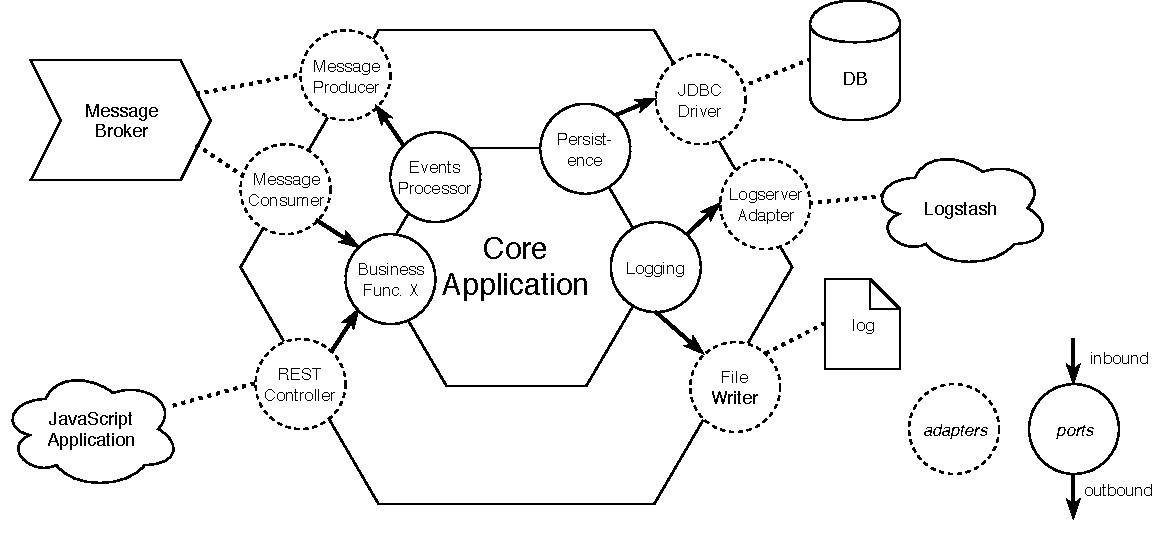
\includegraphics[width=\textwidth]{images/hexagonal_arch.pdf}
    \caption{Hexagonal Architecture}
    \label{fig:hexagonal_arch}
\end{figure}

The \textit{Hexagonal Architecture} was first proposed in 2007 by Alistair Cockburn, one of the co-authors of \textit{The Agile Manifesto}\footnote{https://agilemanifesto.org/}.

It aims to overcome limits of the layered architecture. The business logic is isolated in the centre (\textit{Core Application} in \nameref{fig:hexagonal_arch}) and exposes interfaces called \textit{ports}.

Ports have two directions:
\begin{itemize}
    \item \textbf{inbound} handle the invocations of the business logic from the outer world, usually an \acrlong{API}
    \item \textbf{outbound} is how the business logic interacts with external systems, e.g. a data persistence, logging, message publishers
\end{itemize}

Between a port and an external system is an \textit{adapter}, which bridges the business logic port with the specific technology (e.g., a \acrlong{DAO}). The core application does not depend on the adapters. Therefore it is easy to swap, e.g., a generic \acrshort{ORM} for a custom optimized \acrshort{DAO}.

More than one adapter may be bound to a single port (e.g., the same business logic action is invoked by a message received or by a \acrshort{REST} call).

Decoupling using ports and adapters allows easy extendability without any changes introduced to the business logic. It also makes the core application testable without the need for the surrounding components (e.g., the whole application can be black-box tested without a need for \acrshort{DB})

\subsection{Monolith Architecture}

\acrshort{MSA} in this thesis is often compared to a \textit{monolith} or a \textit{monolithic architecture}. This term is a polyseme --- it is applied to more than one of the four architectural views and has a different meaning in each of them.

Originally it was used in context of the layered architecture (i.e., in the logical view). It was a synonym for the 1-tier logically unstructured code base \cite{professional-asp, wiki-monolith}, usually exhibiting the same poor properties as the \textit{big ball of mud}~\cite{big-ball-mud}.

On the dawn of microservice architecture, it needed to be compared to the traditional single-process application --- so the word monolith received a new meaning. In \cite{ms-today-tomorrow} it is defined as:

\begin{quote}
    A monolith is a software application whose modules cannot be executed independently.
\end{quote}

In this context, \textit{monolith} doesn't have the pejorative connotation, as it often represents the well structured, n-tier application (see \fullref{fig:monolith_vs_microservices}).

In this thesis the word \textit{monolith} is used exclusively with the second meaning.

% % % % % % % % % % % % % % % % % % % % % % % % % % % % % % 
% 
% Literature Review
% 
% % % % % % % % % % % % % % % % % % % % % % % % % % % % % % 

\chapter{Microservice Architecture Literature Review}
\label{sec:literature_review}
This chapter surveys the available literature and other sources of information on the topic of \textit{\acrlong{MSA}}, \textit{evolvability of \acrlong{MSA}} and \textit{application of \acrlong{NS} to software architecture}.

Section \ref{sec:related_work} is a comparison of scope of this thesis to state-of-the-art academic research and industry publications.

The retrieved knowledge is synthesized and critically analyzed in \fullref{sec:msa_analysis}.

% 
% Literature
% 
\section{Available Sources}
Microservices as an architecture style started appearing around year 2013 \cite{ms-fow-new-term-def}. Since then, research is lead by industry and practitioners. Academia is was a long time reluctant to this field (see \fullref{tab:ms_trends}).

A lot of knowledge appeared on the Internet before the science journals and is often referenced in various articles (e.g., \cite{ms-today-tomorrow, ms-taxonomy, ms-sc-collaborative-mdd, ms-sc-measuring}). To track back the original sources and to follow the most recent trends, an unorthodox category of information sources is created --- the community. This category consists of various non-reviewed Internet sources, such as personal blogs or Git repositories. Trustworthiness of those sources was assessed by cross-checking the information, reputation of the author(s), and to a lesser extent medium of publication. 


\subsection{Academic Literature}

Search engines used for the academic sources were: SpringierLink\footnote{https://link.springer.com/}, IEEE Explore\footnote{https://ieeexplore.ieee.org/},  ScienceDirect\footnote{https://www.sciencedirect.com/}, ACM Digital Library\footnote{https://dl.acm.org/}

\begin{table}
\centering
\caption{Number of published articles with keyword \textit{microservices}}
\label{tab:ms_trends}
\begin{tabular}{r|r|r|r|r}
              & \textbf{SpringierLink}  & \textbf{IEEE Explore} & \textbf{ScienceDirect} & \textbf{ACM DL}                \\ 
\hline
\textbf{2013} & 5                       &  1                    & 0                       & 0                             \\ 
\hline
\textbf{2014} & 5                       &  3                    & 0                       & 0                             \\ 
\hline
\textbf{2015} & 30                      & 24                    & 6                       & 7                             \\ 
\hline
\textbf{2016} & 125                     & 76                    & 30                      & 40                            \\ 
\hline
\textbf{2017} & 218                     & 153                   & 53                      & 62                            \\ 
\hline
\textbf{2018} & 350                     & 204                   & 118                     & 65                           
\end{tabular}
\end{table}

- taxonomie





\subsection{Industry Literature}

The book 


\subsection{The Community}

- blogs Fowler,
- github repositories
- 

Due to the last 


% 
% Related Work
% 
\section{Related Work}
\label{sec:related_work}
\subsection{Academic Literature}
\subsubsection*{Normalized System Institute books}
The first published \acrshort{NS} book \cite{ns-recreating} provides a brief discussion of compliance of the \acrfull{SOA} with \acrshort{NS}. Authors note that \acrshort{SOA} may exhibit desired properties of evolvability, but don't provide any further argumentation.

The second \acrshort{NS} book \cite{ns-toward-general-theory} contains plenty of related information:
\begin{itemize}
    \item Chapter \textit{12 Toward Stable Modular Software Architectures} provides a prescriptive design rules for stable software architectures.
    \item Chapter \textit{15 Normalized Elements for Software Architectures} presents essential building blocks of evolvable architectures --- \textit{normalized elements} --- and shows the implementation of those elements on code examples.
\end{itemize}

Content of both chapters is highly relatable to the focus of this thesis. Although the knowledge is not effortlessly applicable to the distinctive domain of \acrlong{MSA}.

\subsubsection*{Science Journals}
The domain of \textit{evolvability of \acrlong{MSA}} seems to be a virgin territory in the scientific journals. Searches performed in databases of respected science publishers yielded exactly zero relevant results. The search results were not always an empty list due to generality of some keywords (e.g., \textit{change} or \textit{distributed system}), but the after closer examination the returned results were all considered irrelevant.

Keywords were all pairs composed of members of two sets:
\begin{itemize}
    \item microservices, microservice architecture, service oriented architecture, distributed systems
    \item evolvability, change, normalized systems
\end{itemize}



\subsection{Industry Literature}



\subsection{The Community}
Bloggers and programmers often consider \textit{evolvability} a virtue. But it is not a~frequently discussed topic and the community does not provide any relevant information on this particular problem.

% % % % % % % % % % % % % % % % % % % % % % % % % % % % % % 
% 
% Microservice Analysis
% 
% % % % % % % % % % % % % % % % % % % % % % % % % % % % % % 
\chapter{Analysis of the~Microservice Architecture}
\label{sec:msa_analysis}

% 
% Design, scope, etc.
% 
\begin{figure}[b]
  \centering
    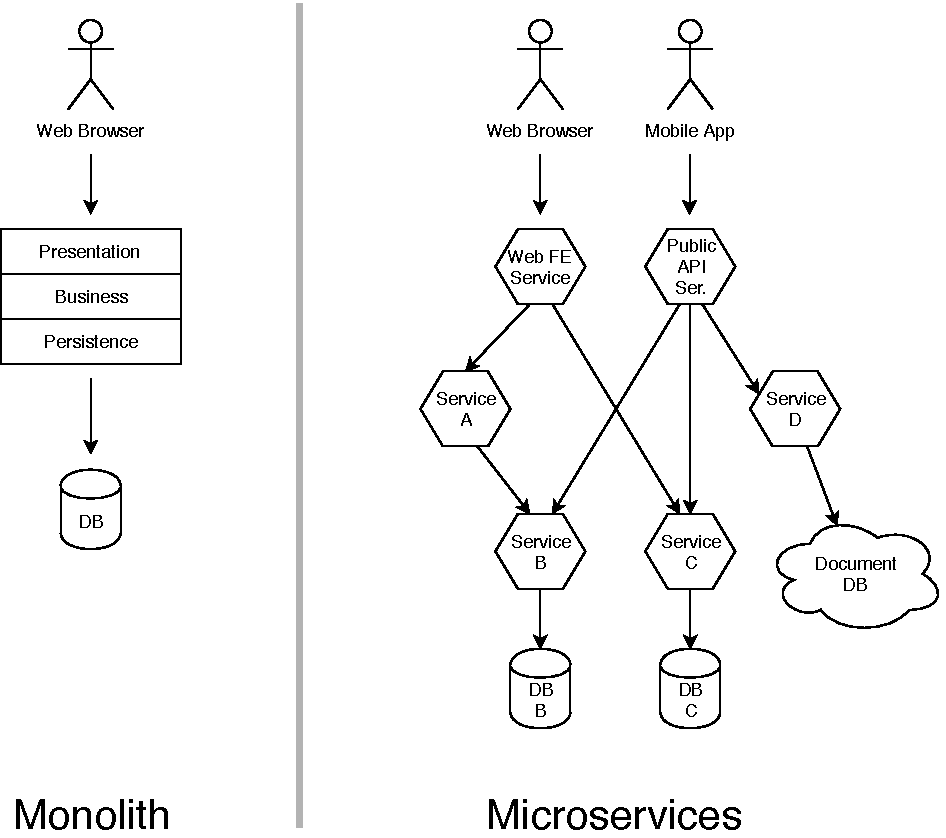
\includegraphics[width=0.7\textwidth]{images/monolith_vs_microservice.pdf}
    \caption{Monolith vs. Microservices Illustrated}
    \label{fig:monolith_vs_microservices}
\end{figure}

Microservice architecture is described in process view --- simply as a collection of processes communicating with each other. Although logical and development views may be organized organized in any way, \acrshort{MSA} strongly endorses one rule: share nothing with others. This extremely radical decoupling allows swift development of independently deployable artifacts.

This architecture style is exploited by leading companies in the online business --- e.g., Amazon, Ebay, Netflix, Spotify, Uber, SoundCloud and many more \cite{ms-who-is-using}. The enterprises praise adoption of this style due to its two crucial features: easy \textit{scalability} to their extreme dimensions \cite{ms-ebay-scalability-best-practices, ms-ebay-ds-scalability, ms-spotify-horizontal-scaling, ms-spotify}, and rapid development of new features --- \textit{evolvability}. Modern enterprises are able to create new functionality on an unprecedented rates - online marketplace Etsy is able to release new features 50 times a day and Amazon deploys new code to production every 11.3 seconds \cite{devops-deploying-hourly}.

%Independence is the essential principle of \acrshort{MSA}. Not only it allows teams to deploy their artifacts independently, it allows them to choose any 3rd party technology they want to use. Teams handle th 
\todo{independence? rozepsat?}

In spite of all the listed advantages, \acrlong{MSA} is no silver bullet. This style adds a lot of obvious as well as hidden complexity --- complicated operations, asynchronous communication, fallacies of distributed computing \cite{devops-fallacies}, changes in organization necessary to deal with \textit{Conway's law} \cite{conways-law}. (More in \fullref{sec:tradeoffs}).

It's not easy to decide when the pros \acrshort{MSA} compensate the cons. Analysis of the proper decision making is too complex to fit in scope of this thesis, but the general rule of thumb is:
\begin{quote}
    Don't even consider microservices unless you have a system that's too complex to manage as a monolith.~\cite{ms-fow-monolith-first}
\end{quote}

\begin{figure}
  \centering
    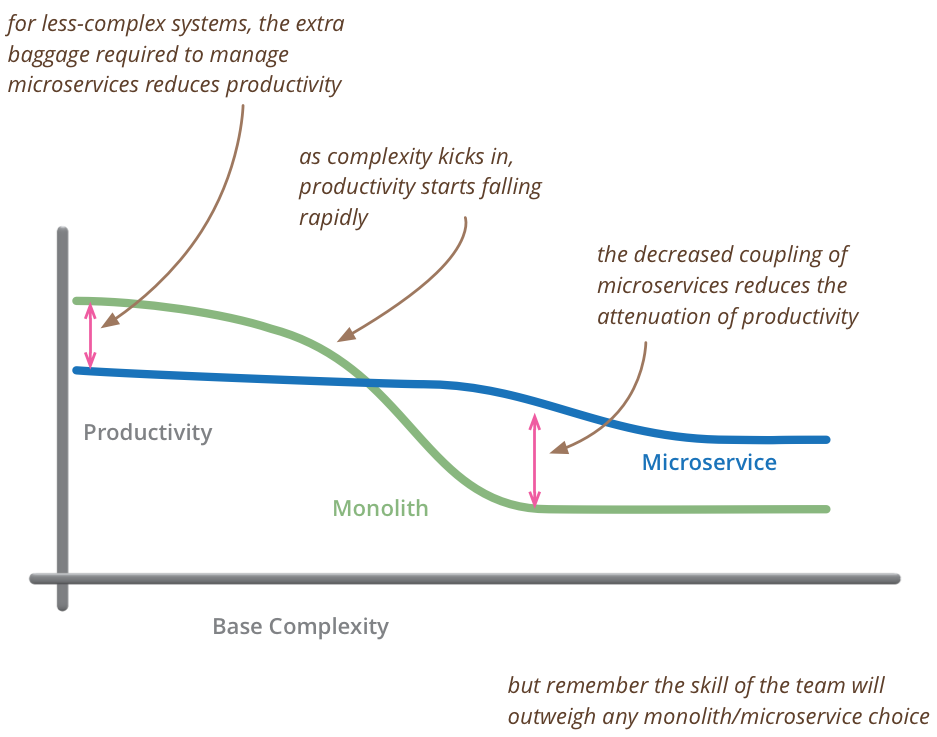
\includegraphics[width=0.7\textwidth]{images/microservices_productivity.png}
    \caption{Monolith vs. Microservices --- Productivity to Complexity ratio~\cite{ms-fow-monolith-first}}
    \label{fig:microservices_productivity}
\end{figure}


\textit{Microservices} is a buzzword now and \textit{since the successful large companies adopted this architecture, it must be the key to their success} --- this is a portrayal of a dangerous phenomenon called \textit{Microservice Envy}. This assumption may lead a lot of \acrshort{RD} departments to unnecessary struggle. The ThoughtWorks company made a website dedicated to monitoring the state-of-the-art of \acrshort{MSA} knowledge and tooling to help other teams to avoid this pitfall.\footnote{https://www.thoughtworks.com/radar/techniques/microservice-envy}


\section{(De)composition of Microservice Application}

This section looks closer on the eminent implications and concerns creating a~\acrlong{MS} application.

\subsection{Microservice scope}
Microservice applications are composed of \textit{microservices}. The preposition \textit{micro} suggests existence of some \textit{milliservices} or \textit{nanoservices}. Or at least that the \textit{microservice} itself should be very small. This might be very misleading interpretation. If we consider the common rule, that the microservice code base should be owned by one cross-functional team \cite{ms-building-ms, ms-evolutionary-arch, ms-fow-new-term-def} with top limit of 8-10 people, the deployed artifact might not be small at all.

\acrshort{MSA} could be used for project starting from scratch (a \textit{greenfield} project), or for splitting a monolithical code base (a \textit{brownfield} project). Regardless of the origin, the recommended first step is always deep analysis of the application domain. The well-known methodology for this purpose is \textit{domain driven design} (\acrshort{DDD}) exquisitely described in \cite{domain-driven-design}.

Based on a particular domain model, the development team can identify real-world components. Each component is responsible for a \textit{business capability} --- in \acrshort{DDD} it is called a \textit{bounded context}. Seams between the bounded contexts are the first candidates for microservice boundaries.

This approach is the essence mentioned in the industry-oriented books \cite{ms-building-ms, ms-evolutionary-arch, ms-patterns, ms-ca} as well as science journals \cite{ms-integrating-with-adaptable-ea, ms-towards-integrated-soa, ms-design-tradeoffs, ms-approaches-to-soa-evolution, ms-self-managing} and many blog posts (e.g., \cite{ms-fow-new-term-def, ms-modelling-with-petter}). Yet, this is the only advice that is given by the many authors of the professional literature. The rest is upon the particular domain, experience of the \acrlong{EA} and the team delivering the service. 

\subsection{Inner vs. Outer Architecture}

\begin{figure}
  \centering
    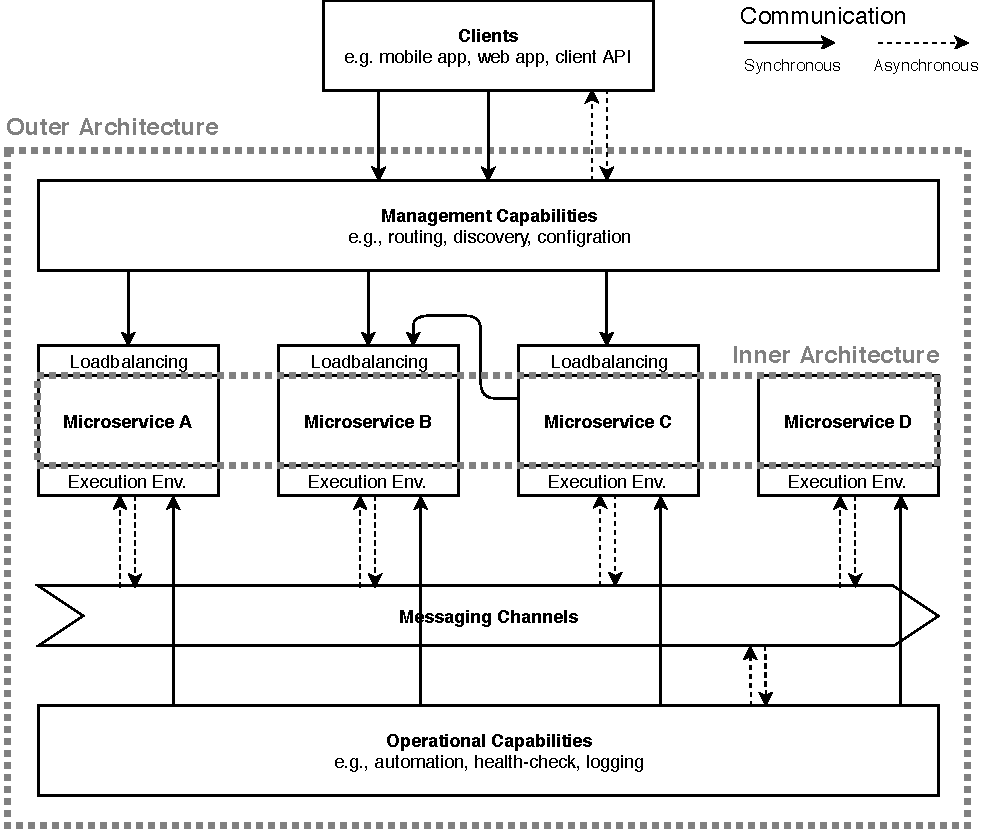
\includegraphics[width=0.7\textwidth]{images/architecture_inner_vs_outer.pdf}
    \caption{Inner vs. Outer Architecture}
  \label{fig:in-vs-out-arch}
\end{figure}

Until now, the \acrshort{MSA} was discussed as a cluster of independently deployed services and communication between them. On the other hand, the resultant artifact was always addressed as one \textit{application} --- that means the services construct an integral system. In order to keep balance between the freedom of the inner workings of a \acrshort{MS} and complexity of operations, another border between \textit{inner} and \textit{outer} architecture must be defined (see fig. The \fullref{fig:in-vs-out-arch}).

The \textbf{outer architecture} includes direct communication between services and other supporting systems (e.g., monitoring and logging), the execution environments (e.g., docker containers or \acrshort{VM}s), networking (including load-balancing, routing etc.) and messaging channels (i.e. message brokers). It doesn't describe just the inter-connections, but more importantly the \textit{contracts} between them (i.e. the \acrshort{API} definitions). 

The \textbf{inner architecture} is everything else --- the internal business logic, the choice of programming language, 3rd party libraries and frameworks (if it's possible to run them in the supported execution environment), the data persistence (everything from \acrshort{ORM} through schema to the choice of \acrshort{DBMS} is hidden from the outer world --- as long as it is able to be executed in the unified environment).

\subsection{Technological diversity}
The freedom of the inner architecture is often considered an advantage of \acrshort{MSA}. It allows developers to \textit{select the best weapons} --- the best programming language, the best 3rd party technology, the most suitable \acrshort{DB} schema. It allows experimentation with all the aspects and that keeps the developers motivated \cite{ms-building-ms, ms-3-pillars}, fosters the culture of innovation \cite{innovation-well-oiled-machine}, reduces the chance of lock-ins for outdated technology \cite{ms-building-ms} and helps keep the whole application loosely coupled (see \ref{sec:strong_boundaries}).

\subsection{Strong Module Boundaries}
\label{sec:strong_boundaries}
A common recommendation in \acrshort{SW} development is to have clearly defined code module boundaries. It's the manifestation of loose coupling and Douglas McIlroy's vision (see \fullref{sec:evolvability_rules}). \acrshort{MSA} is no different.

Respecting the strong module boundaries doesn't depend on the architecture style --- it is possible to create a perfectly modular monolithic app. It is only the matter of developer's discipline.

The \acrlong{MSA} magnifies the need for modularization by its intrinsic features, e.g., separate build artifacts for independent deployment, freedom of choice in technologies or persistence encapsulation.

Therefore, a developer feels much stronger guilt for including code from another service, when he knows the code he \textit{borrows} might be rewritten to completely different programming language without prior notice.

Sometimes the discipline means breaking some established but blindly-followed guidelines and best practices. For example the undisputed \acrfull{DRY} principle must be in context of \acrshort{MSA} be applied only on the microservice level, not across the whole application. 

Authors of the up-to-date industry literature \cite{ms-building-ms, ms-evolutionary-arch, ms-ca} also recommend an extreme caution when creating an internal shared library of common functions and/or data structures (e.g., \acrshort{DTO}s) since it leads to unrestrained coupling and the time invested into creation of such artifacts limits the technological diversity. 

\subsection{Trade-offs of a Distributed Architecture}
\label{sec:tradeoffs}

This section analyses the costs of adoption of the microservice architecture. Every benefit listed in the previous section has a cost of its own. And almost all of them increase the overall complexity of the system.

\subsubsection{Distribution}
\acrshort{MSA} utilizes a distributed system to provide fine-grained modularity. The fact it is distributed bring a lot of complexity and possible unintended consequences. 

L. Peter Deutsch compiled a list called \textit{Fallacies of distributed computing} \cite{devops-fallacies-wiki} in 1994. The list consists of eight false assumptions which must be kept in mind while designing and operating a distributed system: 
\begin{multicols}{2}
    \begin{itemize}
        \item The network is reliable.
        \item Latency is zero.
        \item Bandwidth is infinite.
        \item The network is secure.
        \item Topology doesn't change.
        \item There is one administrator.
        \item Transport cost is zero.
        \item The network is homogeneous.
    \end{itemize}
\end{multicols}

All of the listed fallacies are still valid \cite{devops-fallacies}, although effects of some are were alleviated due to the advance of related technology.

\textbf{The network is reliable.} has a whole \fullref{sec:resilience} dedicated to dealing with this phenomenon.

\textbf{Latency is zero.} \& \textbf{Transport cost is zero.} \& \textbf{Bandwidth is infinite.} have a great impact on applications performance. The ways how to mitigate this are discussed in \fullref{sec:inter-service-communication}.

\textbf{Topology doesn't change.} \& \textbf{The network is homogeneous.} \todo{odkazat na service discovery nebo nejak ukecat}

\textbf{The network is secure.} \& \textbf{There is one administrator.} belong to the application operations domain, therefore are out of scope of this analysis.

\subsubsection{Eventual Consistency}
\begin{figure}
  \centering
    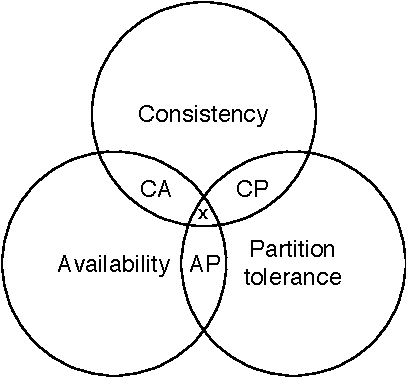
\includegraphics[width=0.5\textwidth]{images/CAP.pdf}
    \caption{CAP Theorem}
    \label{fig:cap}
\end{figure}
The \acrshort{MSA} is a distributed architecture therefore it exhibits implications of the \acrshort{CAP} (also known as Brewer's) theorem \cite{cap-acm}. The theorem states that a distributed data store can't provide more than two out of the following properties:
\begin{itemize}
    \item \textbf{Consistency} --- each read receives the most recent write or an error.
    \item \textbf{Availability} --- each request receives a non-error response, although without a guarantee to contain the most recent write.
    \item \textbf{Partition tolerance} --- the data store responds with an non-error reply despite an erratic number of messages being lost or delayed in communication between nodes.
\end{itemize}

The implications of this phenomenon are known to all users of some of the present-day web applications --- missing updated data, inconsistent notifications counts, etc. That's the nature of distributed architecture: the request to update data is handled by green node, the request for listing the data is handled by blue node. Until the blue and green nodes exchange information, the user is stuck in an \textit{inconsistency window}.

For users, the eventual consistency is just annoying. For a programmers it is a whole lot of added complexity they have to deal with. The logic they've might end up making decisions on inconsistent information. This issue is exceptionally difficult to debug as the numbers of possible situations may rise extremely.

Design patterns guaranteeing the eventual consistency already exist (see \fullref{sec:transaction_management}), but for some use cases it might not be good enough. The \textit{eventuality} will probably never be accepted in mission-critical financial, traffic control and similar systems. Since the \acrshort{CAP} theorem is formally proven, the \acrshort{MSA} will be hardly ever adapted in domains with such requirements.

\subsubsection{Operational Complexity}
By splitting up the monolithic code base, the complexity of the code base itself lowers, but it leaks into the space between the microservices --- into the operations of the application. The number of deployed code artifacts rise; number of \acrshort{DBMS} and NoSQL \acrshort{DB}s rise; load-balancers, message brokers and monitoring and management systems need to be deployed.

The swarm of tiny services is almost impossible to handle one by one. That reinforces the importance of \acrfull{CI} and \acrfull{CD} tools and practices, as well as it enforces the implementation of the DevOps ideas and culture.

Distributed architecture also necessitate additional supporting systems, such as monitoring dashboards and centralized logging. Lack of those systems render almost impossible to trace back a bug in the application.

% 
% Communication patterns
% 

\section{Inter-microservice Communication}
\label{sec:inter-service-communication}

The \textit{inter-microservice communication} is a specialization of a general problem in \acrshort{IT} called \acrfull{IPC}. In the professional literature the discussion of this specialization of the problem usually resorts to even greater specialization of discussing particular problems and patterns (e.g. \acrshort{REST} vs. \acrshort{RPC} or \acrshort{XML} vs. \acrshort{JSON}). An abstract taxonomy was needed \cite{ms-taxonomy}.


The microservice architecture is a distributed architecture, so interprocess communication plays a key role.
\begin{verbatim}
    - direct vs. messaging
    - smart endpoints vs. dumb pipes
\end{verbatim}

\subsection{Interaction Models}
Interaction Models refers to the communication flow among components. Possible values: synchronous, asynchronous.


\subsection{Interaction styles}



It’s useful to first think about the style of interaction between a service and its clients before selecting an IPC mechanism for a service’s API. Thinking first about the inter- action style will help you focus on the requirements and avoid getting mired in the details of a particular IPC technology. Also, as described in section 3.4, the choice of interaction style impacts the availability of your application. Furthermore, as you’ll see in chapters 9 and 10, it helps you select the appropriate integration testing strategy.
There are a variety of client-service interaction styles.



As table 3.1 shows, they can be categorized in two dimensions. The first dimension is whether the interaction is one-to-one or one-to-many:
- One-to-one—Each client request is processed by exactly one service
- One-to-many—Each request is processed by multiple services.
The second dimension is whether the interaction is synchronous or asynchronous:
Synchronous—The client expects a timely response from the service and might even block while it waits.
Asynchronous—The client doesn’t block, and the response, if any, isn’t necessar- ily sent immediately.
Table 3.1 The various interaction styles can be characterized in two dimensions: one-to-one vs one-to- many and synchronous vs asynchronous.
Synchronous —
Asynchronous Publish/subscribe Publish/async responses
The following are the different types of one-to-one interactions:
Request/response—A service client makes a request to a service and waits for a response. The client expects the response to arrive in a timely fashion. It might event block while waiting. This is an interaction style that generally results in services being tightly coupled.
Asynchronous request/response—A service client sends a request to a service, which replies asynchronously. The client doesn’t block while waiting, because the ser- vice might not send the response for a long time.



\subsection{Service Interfaces}
\textcolor{magenta}{Service Interfaces are the different means of specifying contracts (if any) for the communication of microservices [45]. Possible values: formal (defined through a formal contract), tech-tied (the interface is tied to the implemen- tation technology), ad-hoc (defined in a novel language).}


\subsection{Data Exchange Protocol}
Data Exchange are the protocols used to represent the communication. Possible values: REST/HTTP, RPC-alike, message queues, other.

% 
% Transaction management
% 
\section{Transaction management}
\label{sec:transaction_management}
After that I look at the two different ways of coordinating sagas: choreography, where participants exchange events without a centralized point of con- trol, and orchestration, 

\subsection{Two-Phase Commit}
\subsection{Three-Phase Commit}
\subsection{The Saga Pattern}


\section{Deployment \& Operations}
\textcolor{magenta}{Independent Deployment: Simple services are easier to deploy, and since they are autonomous, are less likely to cause system failures when they go wrong.}

\textcolor{magenta}{Deployment encompasses how and where services are actually hosted and deployed. Although the cloud has been adopted as the de-facto platform for microservices [44], there are several alternatives into and out of the cloud.}

\textcolor{magenta}{– Platform can be customized due to privacy, security or business constraints. Possible values: public cloud, private cloud, in-house.}

\textcolor{magenta}{– Management encompasses the responsive reaction to failures and changing environmental conditions, minimizing human intervention [7]. Possible val- ues: built-in cloud services (e.g., AWS Cloudwatch and Autoscaling), third- party services (e.g., Rightscale, New Relic), ad-hoc solutions (i.e., tied to the particular approach).}


microservices CA:
Your microservice system is not just a byproduct of the service components that handle messages at runtime. The system behavior is also a result of the processes and tools that workers in the system use to do their job. In the microservice’s system, this usually includes tooling and processes related to software development, code deployment, maintenance, and product management.
Choosing the right processes and tools is an important factor in producing good microservice system behavior. For example, adopting standardized processes like DevOps and Agile or tools like Docker containers can increase the changeability of your system. In Chapters 4 and 6 we will take a closer look at the processes and tools that can have the biggest impact on a microservices system.

% 
% Persistence
% 
\section{Persistence}




\textcolor{magenta}{Eventual Consistency: Maintaining strong consistency is extremely difficult for a distributed system, which means everyone has to manage eventual consistency.}

\textcolor{magenta}{Data Storage usually integrated multiple services in legacy systems, but in microservices architectures it is mandatory to find seams in the databases and use the right technologies to split them out cleanly \cite{ms-building-ms}. Possible values: SQL, graph-oriented, document-oriented, other.}

- one DB per MS pattern 

One key challenge when using messaging is atomically updating the database and publishing a message. A good solution is to use the Transactional outbox pattern and first write the message to the database as part of the database trans- action. A separate process then retrieves the message from the database using either the Polling publisher pattern or the Transaction log tailing pattern and publishes it to the message broker.



\subsection{Scalability / Elasticity}
\label{sec:scalability}
– Scalability and elasticity refer to the capability to rapidly adjust the overall capacity of the platform by adding or removing resources, also minimizing human intervention [7]. Possible values: vendor-provided, autonomic MAPE loops, configuration servers, other.



\subsection{Availability and Resilience}
\label{sec:resilience}
Successful companies that adapted \acrshort{MSA} always design their systems for failure. 
Netflix has developed a tool called \textit{Chaos Monkey}~\cite{chaos-monkey} that is able to randomly terminate services. They are running this tool in production environment, to be sure the whole system is robust and resilient enough to withstand the erroneous termination of deployed instances.



\textcolor{magenta}{Simply handling both service-level and low-level failures that demand for persistence and recovery techniques [45]. Possible values: resilience patterns, fault injection, error-handling policies, resilience tests, other.}



Of course you can do a great deal to mitigate this problem. Firstly you can increase the granularity of your calls, so you make fewer of them. This complicates your programming model, you now have to think of how to batch up your inter-service interactions. It will also only get you so far, as you are going to have to call each collaborating service at least once.

The second mitigation is to use asynchrony. If make six asynchronous calls in parallel you're now only as slow as the slowest call instead of the sum of their latencies. This can be a big performance gain, but comes at another cognitive cost. Asynchronous programming is hard: hard to get right, and much harder to debug. But most microservice stories I've heard need asynchrony in order to get acceptable performance.

Right after speed is reliability. You expect in-process function calls to work, but a remote call can fail at any time. With lots of microservices, there's even more potential failure points. Wise developers know this and design for failure. Happily the kinds of tactics you need for asynchronous collaboration also fit well with handling failure and the result can improve resiliency. That's not much compensation however, you still have the extra complexity of figuring out the consequences of failure for every remote call.



% 
% External API Design
% 
\section{External API}
\label{sec:ext_api}


% 
% Cross-cutting concerns
%
\section{Cross-cutting concerns}
\subsection{Security}
\begin{verbatim}
    - Sessions auth
    - JWT/token authentication
\end{verbatim}

\missingfigure{JWT vs. Session authentication call diagram}

\subsection{Observability}
\subsubsection{Monitoring}
\subsubsection{Logging}


% % % % % % % % % % % % % % % % % % % % % % % % % % % % % % 
% 
% Towards stable microservices
% 
% % % % % % % % % % % % % % % % % % % % % % % % % % % % % % 

\chapter{Towards Stable Microservice Architecture}
\label{sec:msa_compliance}
\section{Mapping NS Elements to Microservice Architecture}

\todo[inline,size=\Large]{Missing whole chapter}

Separation of Concerns
The Netflix microservice architecture arises because of separation of concerns (SoC) in the engineering team organization. Each team owns a group of services. They own building, operating, and evolving those services, and present a stable agreed interface and service level agreement to the consumers of those services. Invoking Conway’s law, an organization structured with independent self-contained cells of engineers will naturally build what is now called a microservice architecture.


\chapter{Guidelines for Stable Microservice Architecture}
\label{sec:guidelines}
\todo[inline,size=\Large]{Missing whole chapter}

% % % % % % % % % % % % % % % % % % % % % % % % % % % % % % 
% 
% Conclusion
% 
% % % % % % % % % % % % % % % % % % % % % % % % % % % % % % 
\setsecnumdepth{part}
\chapter{Conclusion}
\label{sec:conclusion}
\section{Evaluation of Goals}
\todo[inline,size=\Large]{Missing section}

\section{Thoughts on Utilization}
\todo[inline,size=\Large]{Missing section}
- NS - mathematical 



\section{Future Work}
\todo[inline,size=\Large]{Missing section}

%%%%%%%%%%%%%%%%%%%%%%%%%%%%%%%%%%%%%%%%%%%%%%%%%%%%%%%%%%%%
%%%%%%%%%%%%%%%%%%%%%%%%%%%%%%%%%%%%%%%%%%%%%%%%%%%%%%%%%%%%
%%                                                        %%
%%                    REFERENCES ETC.                     %%
%%                                                        %%
%%%%%%%%%%%%%%%%%%%%%%%%%%%%%%%%%%%%%%%%%%%%%%%%%%%%%%%%%%%%
%%%%%%%%%%%%%%%%%%%%%%%%%%%%%%%%%%%%%%%%%%%%%%%%%%%%%%%%%%%%

\bibliographystyle{iso690}
\bibliography{DP_references}

\setsecnumdepth{all}
\appendix

\printglossary[type=\acronymtype,toctitle=]

\chapter{Contents of enclosed CD}
\begin{figure}
	\dirtree{%
		.1 readme.txt\DTcomment{the file with CD contents description}.
        .1 Figures\DTcomment{source files of figures used in the thesis}.
        .1 Text\DTcomment{thesis text}.
            .2 DP\_Kolarik\_Vincenc.pdf\DTcomment{PDF version of~the~thesis}.
            .2 src\DTcomment{\LaTeX{} source codes of~the~thesis}.
    }

\end{figure}

\listoftodos

\end{document}